%%%%%%%%%%%%%%%%%%%%%%% file template.tex %%%%%%%%%%%%%%%%%%%%%%%%%
%
% This is a general template file for the LaTeX package SVJour3
% for Springer journals.          Springer Heidelberg 2010/09/16
%
% Copy it to a new file with a new name and use it as the basis
% for your article. Delete % signs as needed.
%
% This template includes a few options for different layouts and
% content for various journals. Please consult a previous issue of
% your journal as needed.
%
%%%%%%%%%%%%%%%%%%%%%%%%%%%%%%%%%%%%%%%%%%%%%%%%%%%%%%%%%%%%%%%%%%%
%
% First comes an example EPS file -- just ignore it and
% proceed on the \documentclass line
% your LaTeX will extract the file if required
\begin{filecontents*}{example.eps}
%!PS-Adobe-3.0 EPSF-3.0
%%BoundingBox: 19 19 221 221
%%CreationDate: Mon Sep 29 1997
%%Creator: programmed by hand (JK)
%%EndComments
gsave
newpath
  20 20 moveto
  20 220 lineto
  220 220 lineto
  220 20 lineto
closepath
2 setlinewidth
gsave
  .4 setgray fill
grestore
stroke
grestore
\end{filecontents*}
%
\RequirePackage{fix-cm}
%
%\documentclass{svjour3}                     % onecolumn (standard format)
%\documentclass[smallcondensed]{svjour3}     % onecolumn (ditto)
\documentclass[smallextended]{svjour3}       % onecolumn (second format)
%\documentclass[twocolumn]{svjour3}          % twocolumn
%
\smartqed  % flush right qed marks, e.g. at end of proof
%
\usepackage{listings}
\usepackage{graphicx}
\usepackage{longtable}
\usepackage{hyperref}
\usepackage{booktabs}
\usepackage{color}

\definecolor{commentcolour}{rgb}{0.4,0.4,0.4}
\definecolor{keywordcolour}{rgb}{0.8,0.4,0.4}
\definecolor{stringcolour}{rgb}{0.1,0.1,0.5}

\lstset{
    basicstyle=\footnotesize,
%  captionpos=b,                    % sets the caption-position to bottom
    language=Python,                 % the language of the code
    showstringspaces=false,          % underline spaces within strings only
    stringstyle=\color{stringcolour},     % string literal style
    commentstyle=\color{commentcolour},    % comment style
    keywordstyle=\color{keywordcolour}\bfseries,       % keyword style
}

% \usepackage{mathptmx}      % use Times fonts if available on your TeX system
%
% insert here the call for the packages your document requires
%\usepackage{latexsym}
% etc.
%
% please place your own definitions here and don't use \def but
% \newcommand{}{}

\newcommand{\D}{...}
\newcommand*{\affaddr}[1]{#1}
\newcommand*{\affmark}[1][*]{\textsuperscript{#1}}

%
% Insert the name of "your journal" with
% \journalname{myjournal}
%
\begin{document}

\title{A comprehensive framework to capture the arcana of neuroimaging
analysis%\thanks{Grants or other notes
%about the article that should go on the front page should be
%placed here. General acknowledgments should be placed at the end of the article.}
}

%\titlerunning{Short form of title}        % if too long for running head

\author{
	Thomas G. Close\affmark[1,2]\and
	Phillip G. D. Ward\affmark[1,3,4] \and
	Francesco Sforazzini\affmark[1] \and
	Wojtek Goscinski\affmark[6] \and
	Zhaolin Chen\affmark[1,5] \and
	Gary F. Egan\affmark[1,3,4]
}

\authorrunning{
        Thomas G. Close \and
	Phillip G. D. Ward  \and
	Francesco Sforazzini  \and
	Wojtek Goscinski  \and
	Zhaolin Chen  \and
	Gary F. Egan  \and} % if too long for running head

\institute{
	Thomas G. Close \at
	 \email{tom.close@monash.edu} \\ \\
         \affaddr{\affmark[1]Monash Biomedical Imaging, Monash University, Melbourne, Australia} \\
         \affaddr{\affmark[2]Australian National Imaging Facility, Australia} \\
         \affaddr{\affmark[3]Australian Research Council Centre of Excellence for integrative Brain Function, Melbourne, Australia} \\
         \affaddr{\affmark[4]Monash Institute of Cognitive and Clinical Neurosciences, Monash University, Melbourne, Australia} \\
         \affaddr{\affmark[5]Department of Electrical and Computer Systems Engineering, Monash University, Melbourne, Australia} \\
         \affaddr{\affmark[6]Monash eResearch Centre, Monash University, Melbourne, Australia} \\
}

%\date{Received: date / Accepted: date}
% The correct dates will be entered by the editor


\maketitle

\begin{abstract}
Insert your abstract here. Include keywords, PACS and mathematical
subject classification numbers as needed.
\keywords{First keyword \and Second keyword \and More}
% \PACS{PACS code1 \and PACS code2 \and more}
% \subclass{MSC code1 \and MSC code2 \and more}
\end{abstract}

\section{Introduction}
\label{intro}

Despite the availability of well-established neuroimaging analysis
packages \cite{cox_afni:_1996,smith_advances_2004,friston_statistical_2007,tournier_mrtrix:_2012}, the arcana of neuroimaging analysis is substantial due to
the range of available tools, tuneable parameters, and imaging sequences
involved \cite{cusack_automatic_2015}. The distribution of complete
``end-to-end'' workflows, from acquired data to publication results, is
necessary for routine reproduction because of the effort required to
accurately exactly reimplement such analyses \cite{kennedy_neuroimaging_2018}. It is also
difficult to adapt existing workflows to new studies without detailed
knowledge of their design. Therefore, flexible, portable and complete
workflows are important to promote reproduction and code reuse in
neuroimaging research.

A barrier to designing portable and complete workflows is the
heterogeneity of data storage conventions \cite{marcus_extensible_2007,das_loris:_2012,gorgolewski_brain_2016}.
To address this, the emerging Brain
Imaging Data Standard (BIDS) \cite{gorgolewski_brain_2016} provides a way
to standardise the storage of neuroimaging data in file system
directories. BIDS specifies strict file and directory naming
conventions, which facilitate the design of portable \emph{BIDS Apps}
(https://bids-apps.neuroimaging.io). However, for research groups with
sufficient informatics support, software-managed repositories \cite{marcus_extensible_2007,das_loris:_2012} can provide additional features, such as
flexible access-control and automated pipelines. Therefore, for
published workflows, the choice of repository should be transparent in
order to maximise their audience.

While neuroimaging analyses are generally amenable to standardisation
\cite{kennedy_neuroimaging_2018}, minor modifications are often required to accommodate
idiosyncrasies of the acquisition protocols in use at different sites
\cite{esteban_fmriprep:_2018}. Therefore, workflows may require conditional
logic in construction or execution to be portable. Nipype is a flexible
Python framework for neuroimaging analysis in which workflows are
constructed programmatically in Python \cite{gorgolewski_nipype:_2011}.
Programmatic construction allows for rich control-flow logic that is not
readily available in alternative workflow frameworks \cite{cusack_automatic_2015,achterberg_fastr:_2016,amstutz_common_2016}, and has been used
to implement workflows that are robust to differences in fMRI protocols
across a large number of sites \cite{esteban_fmriprep:_2018}.

The trend towards large multi-site and multi-contrast datasets collected
over a number of years \cite{van_essen_human_2012,thompson_enigma_2014,sudlow_uk_2015}
presents additional challenges to workflow design.
Analysis packages are constantly being developed and improved, so the
state-of-the-art workflow for a particular analysis can change over
time. Therefore, it is challenging to ensure workflows are applied
consistently over the course of long studies \cite{cusack_automatic_2015}.

While analysis workflows for different contrasts and modalities are
typically implemented independently, they can share common processing
steps (e.g. non-linear registration to standard space, surface
parcellation) and their outputs may need to be integrated to produce
publication results. For large scale studies, which are typically
processed on the cloud or high-performance computing (HPC) clusters,
rerunning common segments can lead to significant increases in
computation time and therefore project cost. In addition, duplication of
processing segments increases time for manual quality control (QC),
making the reuse of intermediate derivatives a practical requirement for
some large studies \cite{schreiber_using_2018}.

To maximise the reusability of neuroimaging workflows and avoid frequent
reimplementation of standard analyses, workflow implementations should
be flexible, extensible and applicable to a wide range of storage
systems. In addition, in order to promote routine reproduction of
neuroimaging studies, published workflow implementations should include
the complete procedure, from acquired data to publication results.
However, ensuring workflow implementations are flexible, portable and
complete adds a high degree of complexity and effort to the design
process.

Our objective was to extract common elements of repository-centric
workflow design into an abstract framework to make it practical to
implement flexible, portable and complete workflows for a wide range of
neuroimaging analyses. \emph{Abstraction of Repository-Centric ANAlysis
(Arcana)} \\(\href{http://arcana.readthedocs.io}{http://arcana.readthedocs.io} is a Python framework for
designing complex workflows in which modular Nipype pipelines operate on
data stored in various repositories. Intermediate derivatives are
derived on demand, checking against stored provenance for required
updates. Analyses can be applied to XNAT, BIDS and plain-directory
repositories, and using Nipype's execution plugins, run on workstations
or be submitted as batch jobs to HPC schedulers. Arcana's architecture,
with programmatic workflow construction---yet clear delineation between
analysis design and application---facilitates the implementation of
complex workflows that are portable and complete.

The utility of the Arcana framework is demonstrated by the
implementation of analysis suites for T1, T2* and diffusion weighted MRI
(dMRI) data and the application of dMRI tractogram \cite{tournier_mrtrix:_2012} and
composite vein image \cite{ward_combining_2018} workflows to data collected from a
healthy subject.

\section{Methods}
\label{methods}

\subsection{Framework overview}
\label{framework-overview}

The separation of analysis design and application in the Arcana
framework follows the conceptual divide between classes and objects in
Object-Oriented (OO) software design. \emph{Study} classes encapsulate
imaging data with the suite of analysis methods that can be performed on
them, and, in the basic case, are specialised for a specific imaging
contrast or modality. Study objects apply the analysis suite defined in
the Study class to a specific dataset.

The set of acquired data, the derivatives that can be derived from it,
and methods that construct pipelines to derive the derivatives, are
linked together by the \emph{data specification} \emph{table} of the
Study class (Figure 1). Likewise, free parameters used in pipeline
construction are defined in the class' \emph{parameter specification}
\emph{table}. Class inheritance can be used to specialise analysis
suites by overriding pipeline constructor methods or entries in the
specification tables. Analysis suites for multi-modal data can be
implemented by combining multiple Study classes in \emph{MultiStudy}
classes\emph{.}

\begin{figure*}
  \begin{center}
    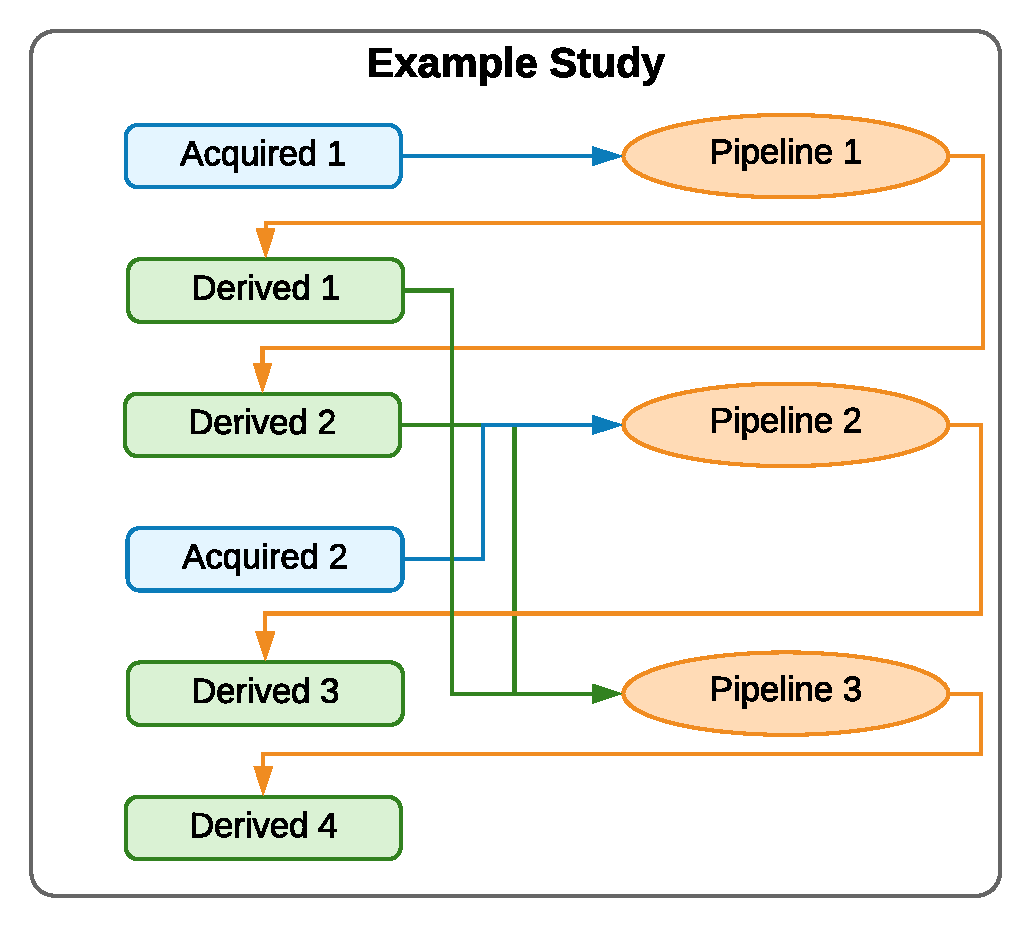
\includegraphics[width=0.55\textwidth]{figures/example_study}
  \caption{Example study. Blue boxes represent acquired (input)
data (filesets or fields) stored in a repository and green derivatives
from that data stored alongside the original data. Orange ovals are
pipelines that operate on data in the repository to derive the
derivatives. Arrows represent data flows, i.e., inputs and outputs to
pipelines}
  \end{center}
\label{fig:example_study}
\end{figure*}

Analysis methods are applied to a specific dataset by instantiating an
appropriate Study class and requesting a derivative listed in the class'
data specification table. At instantiation, a Study object is passed
references to \emph{Repository} and \emph{Processor} objects, which
define how and where data is stored and processed. When a derivative is
requested, a Study object queries the repository for intermediate
derivatives that can be reused before constructing a workflow to produce
the requested derivative. Workflows are executed in the computing
environment specified by the Processor object and their products are
stored back in the repository for reuse by subsequent analyses (Figure
2). Input data to the study are also stored in the repository, and are
matched against entries in the class' data specification table using
criteria defined in \emph{Selector} objects passed to the Study object
at instantiation.

\begin{figure*}
  \begin{center}
    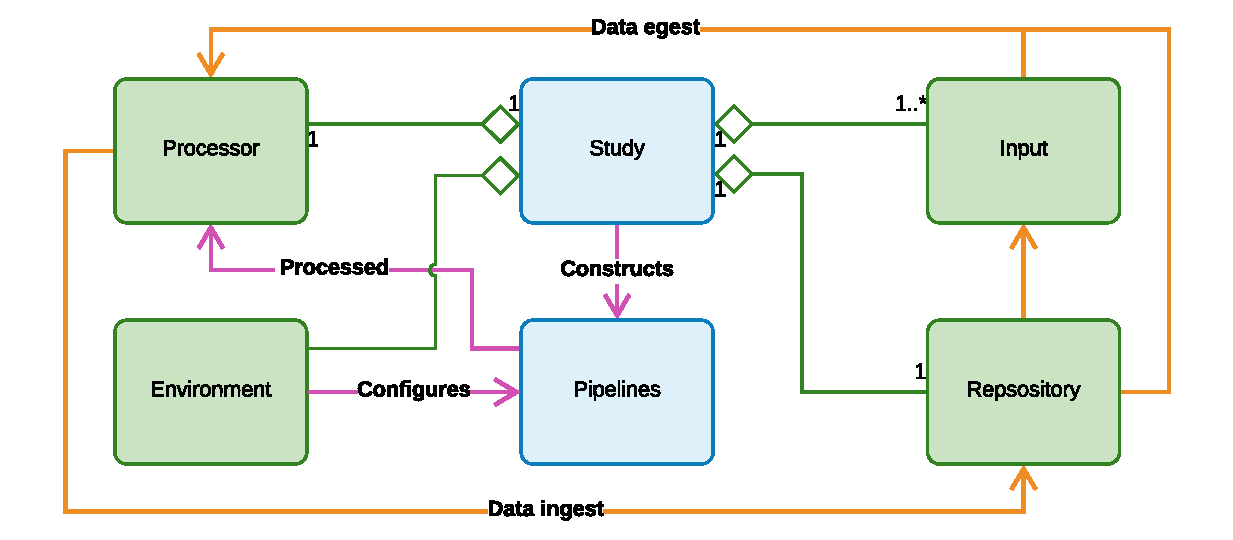
\includegraphics[width=0.9\textwidth]{figures/simplified_arcana_uml}
  \caption{Unified Modelling Language (UML) diagram
of information flow in the Arcana framework. Boxes: Python classes,
blue=analysis-design, green=analysis-application. Arrows: orange=data,
magenta=workflow description, diamond=aggregated-in. Study classes
construct analysis pipelines, which are sent to the \emph{Processor} to
be processed. Input data is selected by \emph{Selector} objects and
pulled to the compute environment to be processed along with existing
intermediate derivatives. After the derivatives are pushed back to the
repository.}
\end{center}
\label{fig:simple_uml}
\end{figure*}

\subsection{Analysis design: Study classes}
\label{analysis-design-study-classes}

Study classes encapsulate a study dataset (i.e. data collected across
multiple subjects using the same acquisition protocol) with the suite of
analytical methods that can be applied to the dataset. The hierarchy of
a study dataset is assumed to have two levels, \emph{subjects} and
\emph{sessions}, with each session for each subject corresponding to a
specific \emph{visit}, e.g. timepoint in longitudinal study. Derivatives
can be created at any point in this hierarchy: per-session, per-subject,
per-visit and per-study. Iteration over subjects and visits is handled
implicitly by the framework. All Study classes must inherit from the
\emph{Study} base class and be created by the \emph{StudyMetaClass}
metaclass or subclasses thereof.

\subsubsection{Data and parameter specification
tables}
\label{data-and-parameter-specification-tables}

At the heart of each Study class is the data specification table, which
specifies both the input and output data of the analysis, and all the
stages in between. There is a one-to-one relationship between entries in
the data specification table and data that is stored in the repository
or will be stored if and when it is derived. Which intermediate
derivatives to include in the data specification table, and therefore
store in the repository, is left to the discretion of the researcher
designing the analysis. However, as a general rule, derivatives that
require manual QC or are likely to be reused between different branches
of analysis should be included in the table.

Data specified in the data specification table can be of either a
\emph{fileset} or \emph{field} type. Filesets represent single files,
header and data file pairs, or sets of related files typically contained
within single directories (e.g. a multi-volume DICOM dataset). Fields
represent a single integer, floating point value or character string
type. Each Fileset references a \emph{FileFormat} object, which
specifies the formats of the files in the set. File formats are
explicitly registered by the researcher at design time using the
\emph{FileFormat.register(format)} class method to avoid conflicts where
the same extension is used for different formats in different contexts.

Fileset and field specifications are passed to the data specification of
a Study class via the \emph{add\_data\_specs} class attribute as a list
of named \emph{FilesetSpec} and \emph{FieldSpec} objects (Figure 3).
Specifications for acquired data (i.e. input data to the study) are
distinguished from derived data by using the \emph{AcquiredFilesetSpec}
and \emph{AcquiredFieldSpec} subtypes. However, the distinction is
fluid, with derived specifications able to be overridden by acquired
specifications in subclasses or MultiStudy classes, and vice-versa, or
passed inputs when the class is instantiated.

\begin{figure}
\lstinputlisting[language=Python, firstline=2, lastline=57]{listings/example_study.py}
\caption{Example data and parameter specifications. The data
specification specifies two ``acquired'' file sets, `one' and `ten' and
ten derived file sets that can be derived from them, at least
indirectly. Each derived data spec, specifies the name of the pipeline
constructor that creates the pipeline that derives them. Parameter
specifications specify a name and default value for free parameters of
the Study class}
\label{list:data_spec}
\end{figure}

Both acquired and derived data specifications have a \emph{frequency}
attribute which specifies where the data sits in the hierarchy of the
dataset and can take the values \emph{per\_session},
\emph{per\_subject}, \emph{per\_visit} or \emph{per\_study}. In
addition, derived specifications are passed the name of a method in the
class that constructs the pipeline to derive them. Therefore, while a
pipeline can have multiple outputs, each derivative is derived by only
one pipeline.

For fileset specifications that correspond to a known type in the BIDS
standard, a \emph{BidsSelector} or \emph{BidsAssociatedSelector} can be
provided to the \emph{bids} keyword arg of the spec. BidsSelector
specifies a primary scan in the BIDS standard using its type, modality
and optional run number. BidsAssociatedSelector is used to select
associated files, such as field maps and diffusion encoding matrices.
When passing a BidsSelector to a FilesetSpec the \emph{run} keyword
argument of the selector is typically not set, so it can be read from
the \emph{bids\_run} attribute of the Study. This allows the Study class
to be applicable to any BIDS run.

Similar to data specifications, parameter specifications are included in
the Study class by providing a list of \emph{ParameterSpec} objects to
the \emph{add\_parameter\_specs} class attribute. ParameterSpec objects
are initialised with a name and default value. Special parameters that
specify a qualitative change in the analysis, for example using ANTs
registration \cite{avants_reproducible_2011} instead of FSL registration \cite{smith_advances_2004}, are specified by the \emph{SwitchSpec} subtype.
SwitchSpecs take a name, default value and a list of accepted values at
initialisation.

\subsubsection{Workflow design}
\label{workflow-design}

Analysis workflows are implemented in Arcana as a series of pipelines
that each perform a unit of the analysis (e.g. registration, brain
extraction). Each pipeline is in turn constructed from a (typically
small) graph of Nipype nodes, with each node wrapping a stand alone tool
(e.g. FSL's FLIRT) or analysis package function (e.g. SPM's \emph{coreg}
tool).

Pipelines are included in the analysis suite of a Study class by
defining a method in the class that constructs and returns a
\emph{Pipeline} object, and referencing that method in the class' data
specification table. Pipeline objects are thin wrappers around Nipype
workflows, which manage the namespaces of the workflow nodes, and should
be created in constructor methods using the \emph{Study.new\_pipeline}
method (Figure 4).

\begin{figure}
\lstinputlisting[language=Python, firstline=58, lastline=108]{listings/example_study.py}
\caption{Example pipeline constructor method. Pipelines are
created using the \emph{create\_pipeline} method of the Study class.
Pipeline objects are thin wrappers around Nipype workflows to allow for
namespace management}
\label{list:pipeline_constructor}
\end{figure}

At instantiation (via the new\_pipeline method) a Pipeline is passed the
following arguments:

\begin{itemize}
\item
  \begin{quote}
  A name for the pipeline
  \end{quote}
\item
  \begin{quote}
  The inputs to the pipeline
  \end{quote}
\item
  \begin{quote}
  The output specifications the pipeline
  \end{quote}
\item
  \begin{quote}
  Description of the pipeline
  \end{quote}
\item
  \begin{quote}
  A list of scientific references the analysis was informed by
  \end{quote}
\item
  \begin{quote}
  Keyword arguments passed directly from the pipeline constructor method
  \end{quote}
\end{itemize}

Inputs and outputs refer to entries in the data specification table and
specify the file formats (fileset) or data type (field) that the input
is expected in, or the output will be returned in. If this
format/data-type differs from that specified in the data specification
table then an implicit conversion will be performed when the pipeline is
executed, thereby making data conversion transparent to the researcher.
Every pipeline constructor should take only wildcard keyword arguments
(i.e. **kwargs), which should be passed directly through to the
new\_pipeline method to enable modification of the pipeline namespace by
overriding methods in subclasses.

The syntax for workflow graph construction in Arcana is inspired by the
proposed format for Nipype v2.0
(\href{http://github.com/nipy/nipype/issues/2539}{http://github.com/nipy/nipype/issues/2539}),
and will be updated as Nipype v2.0 is developed and upstream
functionality becomes available. Workflow nodes are created from Nipype
interfaces using the \emph{add(name, interface)} method of the
Pipeline should be used. Once created, the inputs of the node can be set
explicitly via the node's \emph{inputs} attribute, connected to other
nodes with the \emph{connect(out\_node, out\_node\_output,
in\_node, in\_node\_input)} method, or connected to inputs of the
pipeline. Pipeline inputs and outputs are connected to nodes using the
\emph{add\_input(spec\_name, node, node\_input)} and
\emph{add\_output(spec\_name, node, node\_output)} methods,
respectively.

Any external software packages required by a node should be referenced
in the \emph{requirements} keyword argument as a list of
\emph{Requirement} objects when the node added to the pipeline. These
requirements can be used by the Processor to configure environment
modules \cite{furlani_modules:_1991} if present, to ensure the required software
packages are available. Similarly, the expected memory requirements and
wall time for the node execution should be provided as keyword args,
\emph{memory}, and \emph{wall\_time}, so they can be inserted into job
scripts submitted to schedulers by HPC Processors.

Iteration over subjects and visits is handled implicitly by Arcana and
depends on the frequency of the pipeline's inputs and outputs. To create
a summary derivative (i.e. frequency != \emph{per\_session}) from more
frequent data a join node is used. Join nodes that join over subjects or
visits are created with \emph{add}\_\emph{join\_subjects(name,
interface, joinfield)} and \emph{add\_join\_visits(name,
interface, joinfield)} respectively. As in the underlying Nipype, the
\emph{joinfield} argument specifies which inputs of the receiving node
to join into lists. If direct access to the subject or visit IDs is
required by a node they can be connected to the implicit iterator nodes
with \emph{connect\_subject\_id(node, name)} and
\emph{connect\_visit\_id} respectively. Note that expansion
over iterator sources is handled implicitly by Nipype when nodes with
different iterators are connected to a downstream node.

Study parameters can be accessed during pipeline construction with the
\emph{parameter(name)} method. If conditional logic is included in
the workflow construction that alters the pipeline inputs, outputs or
parameters then it should be controlled by a switch instead of a
parameter. The analysis branch designated by a switch value should be
tested with \emph{branch(name, ref\_value)} method.

\subsubsection{Extension and specialisation by class inheritance}
\label{extension-and-specialisation-by-class-inheritance}

Because Arcana analyses are implemented as Python classes, class
inheritance can be used to specialise existing analyses.

Pipeline constructors can be overridden in subclasses like any Python
method. Typically the overriding method will call the superclass method
to construct a base Pipeline, apply modifications and return the
modified Pipeline. In this scenario, references to the data
specification in the superclass method can be mapped onto different
entries in the subclass by passing a dictionary containing the maps to
the \emph{name\_map} keyword argument of pipeline constructor in the
superclass.

Instead of setting the class attributes directly, the data and parameter
specifications are set by the metaclas\emph{s}, in order to combine with
specifications from base classes. The combined data and parameter
specifications are constructed by visiting the class' bases in reverse
method resolution order (MRO) and adding specifications from their
\emph{add\_data\_specs}, \emph{add\_parameter\_specs} attributes,
overriding previously added specifications with matching names. Note
that in this scheme, specifications can only be appended or overridden
but not removed by Study subclasses so as not to break workflows
inherited from base classes.

\subsubsection{Implementing multi-modal
studies}
\label{implementing-multi-modal-studies}

While basic Study classes are typically associated with single image
modality or contrast, the analysis suites implemented by them can be
integrated into multi-modal analysis by aggregating multiple Study
classes (sub-studies) in a \emph{MultiStudy} class. Analysis suites are
integrated by joining the data specification tables of the sub-studies
of a MultiStudy class. Entries in specification tables of sub-studies
are joined by mapping them to a common entry in the specification table
of the MultiStudy (Figure 6). This enables derivatives from one
sub-study (e.g. brain extracted T1-weighted anatomical) to be referenced
by workflows of other sub-studies (e.g. anatomically constrained dMRI
tractography).


\begin{figure*}
  \begin{center}
    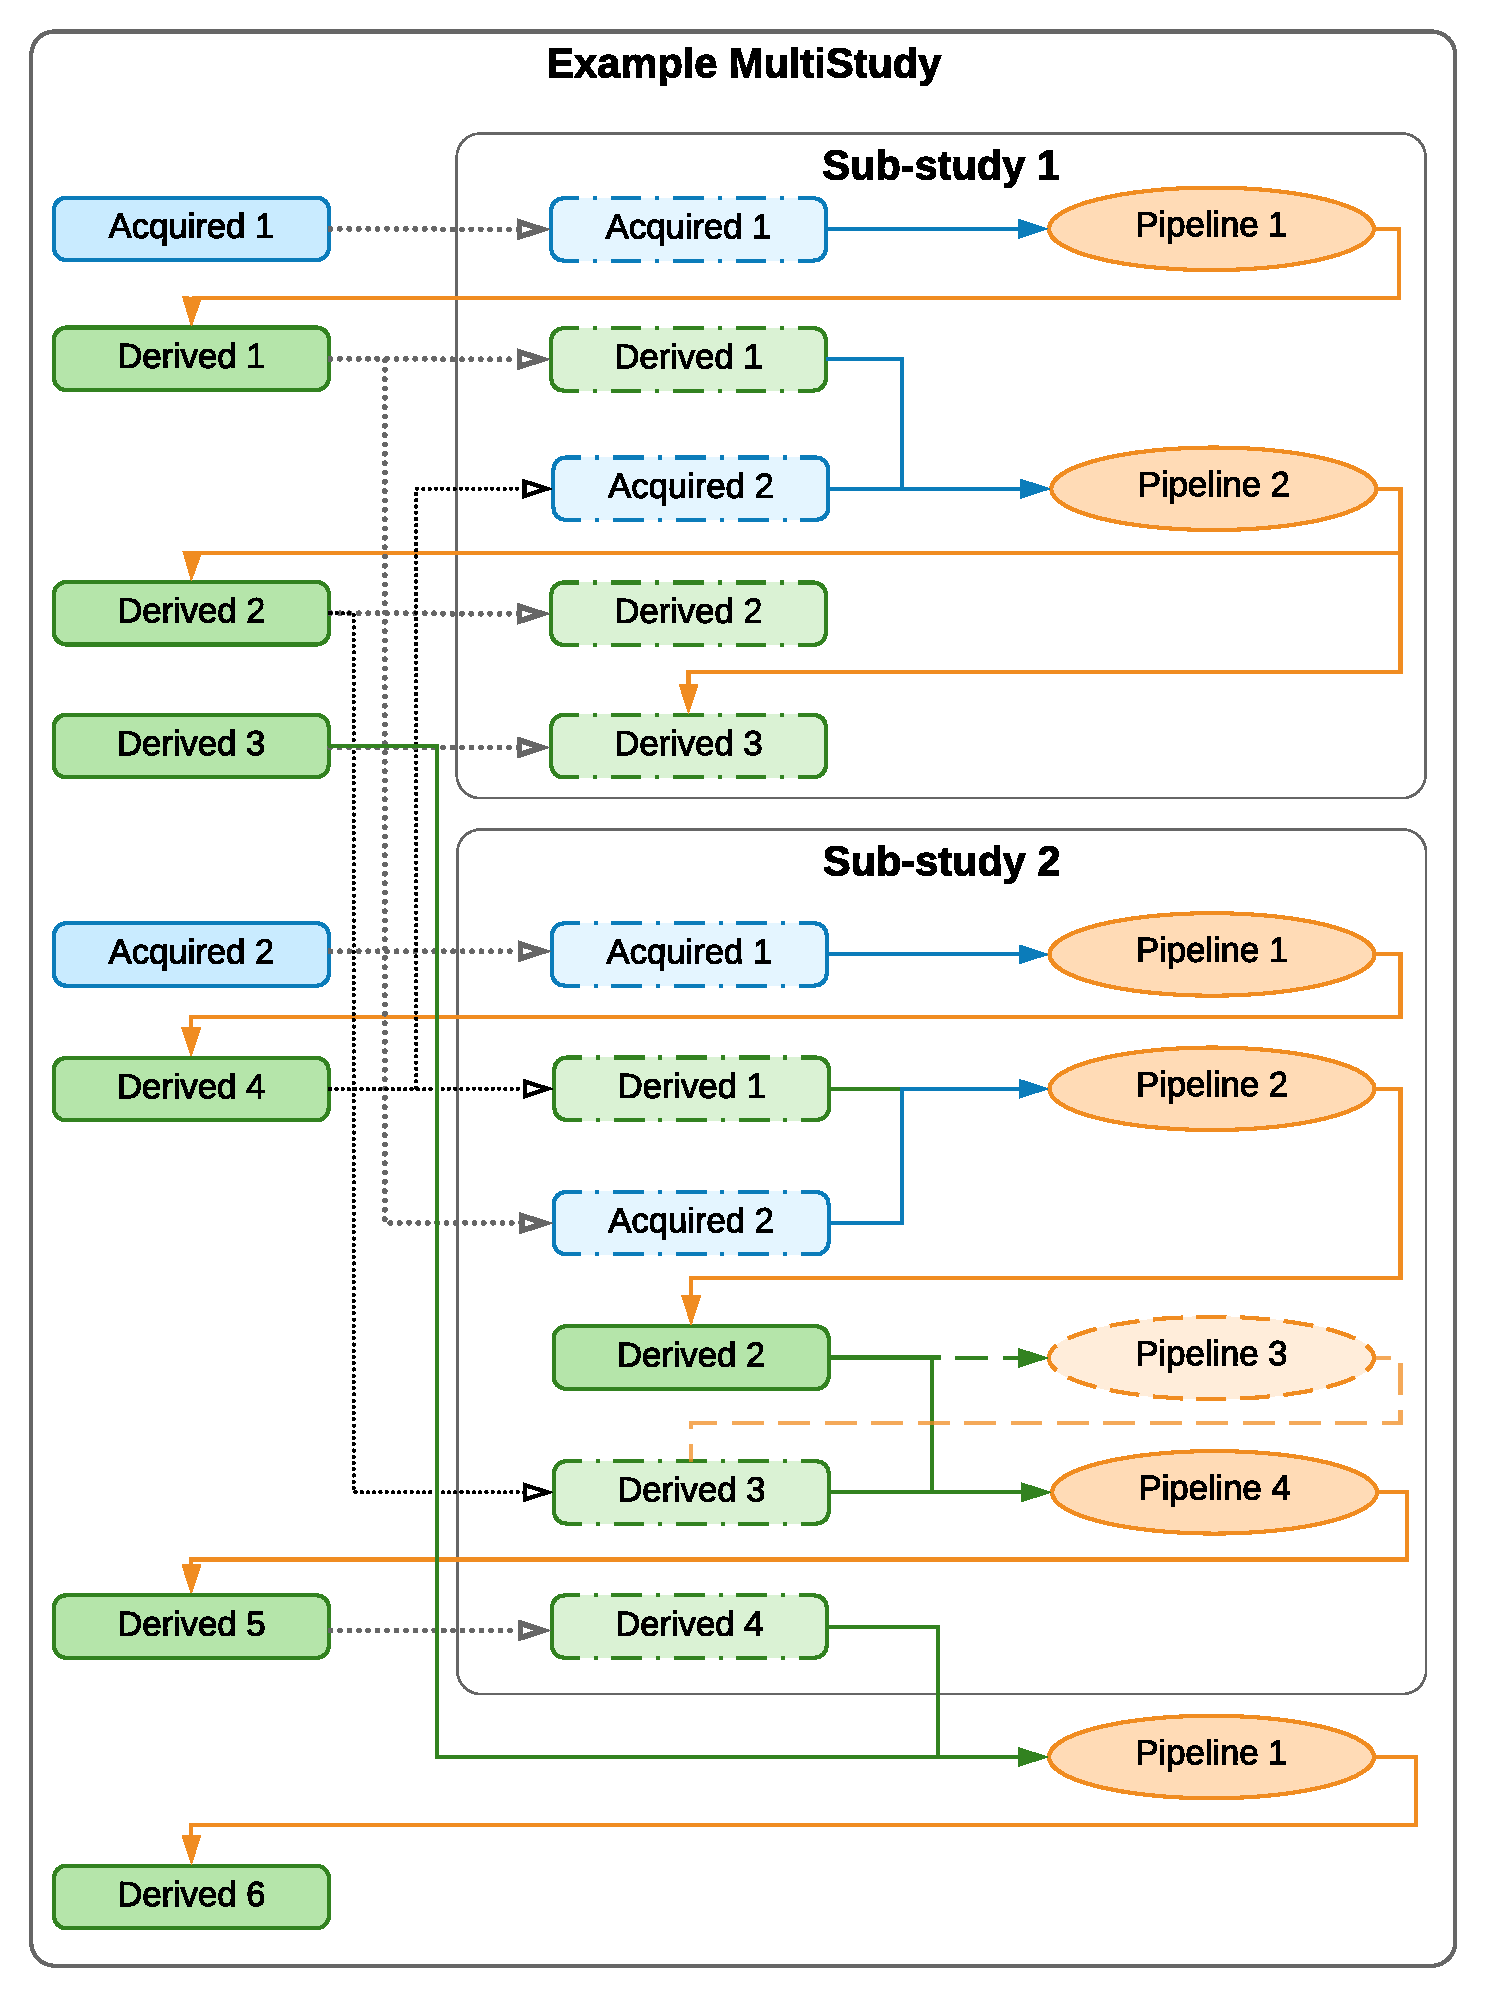
\includegraphics[width=0.775\textwidth]{figures/example_multi_study}
  \caption{Example MultiStudy. Blue boxes represent acquired
(input) data (filesets or fields) and green derivatives. Orange ovals
are pipelines. Blue and green arrows: acquired and derived inputs to
pipelines, respectively. Orange arrows: outputs of pipelines. Dashed
boxes represent data specifications in a sub-study that are present in
the global namespace and mapped into the sub-study space, and dotted
arrows the mappings. Sub-studies are linked by mapping the same data
spec in the global space onto data specifications the multiple sub-study
namespaces (e.g. \emph{Derived 1, 2 \& 3}). There are no restrictions
between mapping acquired and derivative specifications: both acquired
and derivative specifications can be mapped onto acquired data or
derivative specifications in sub-studies. If a spec in the global spaced
is mapped onto a derivative spec in the sub-study space, then the
pipeline that generates that derivative in the sub-study will not run
unless it generates other required derivatives (e.g. \emph{Pipeline 3} in
\emph{Sub-Study 2})}
\end{center}
\label{fig:example_multi_study}
\end{figure*}

All MultiStudy classes must inherit from the Multi\emph{Study} base
class and be created by the Multi\emph{StudyMetaClass} metaclass or
subclasses thereof. As in the case of subclassing the standard Study
class, additional data and parameter specifications can be added to the
class via \emph{add\_data\_specs} and \emph{add\_parameter\_specs}
respectively for additional analysis not included in the sub-studies.

Sub-studies are aggregated in the \emph{sub-study} \emph{specification
table} of a MultiStudy class via a list of \emph{SubStudySpec} objects
in the \emph{add\_sub\_study\_specs} class attribute, in the manner of
data and parameter specifications. A SubStudySpec consists of a name, a
Study class, and a \emph{name map} dictionary\emph{.} The name map
dictionary maps data and parameter specification names from the
namespace of the MultiStudy class to the namespace of the Study class.

Entries in the specification tables of sub-study classes that are not
referenced in the sub study's name map are implicitly mapped to the
MultiStudy namespace in the construction of the MultiStudy class by the
metaclass using the name of the sub-study as a prefix. If the spec is a
derivative then the pipeline constructor used to derive it is also
mapped into the MultiStudy namespace. For example, \emph{derived1} in
\emph{sub\_study2} would be mapped to \emph{sub\_study2\_derived1} along
with the method \emph{sub\_study2\_pipeline1}.

\hypertarget{analysis-application-study-instances}{%
\subsection{Analysis application: Study
instances}\label{analysis-application-study-instances}}

To apply the analysis blueprint specified in a Study class to a specific
dataset, an instance of the Study class is created with details of where
the data is stored (the \emph{Repository}) and the computing environment
available to process it (the \emph{Processor}). A Study object controls
the construction of analysis workflows, the execution of the workflows,
and the flow of data to and from the repository (Figure 7).

\begin{figure*}
  \begin{center}
    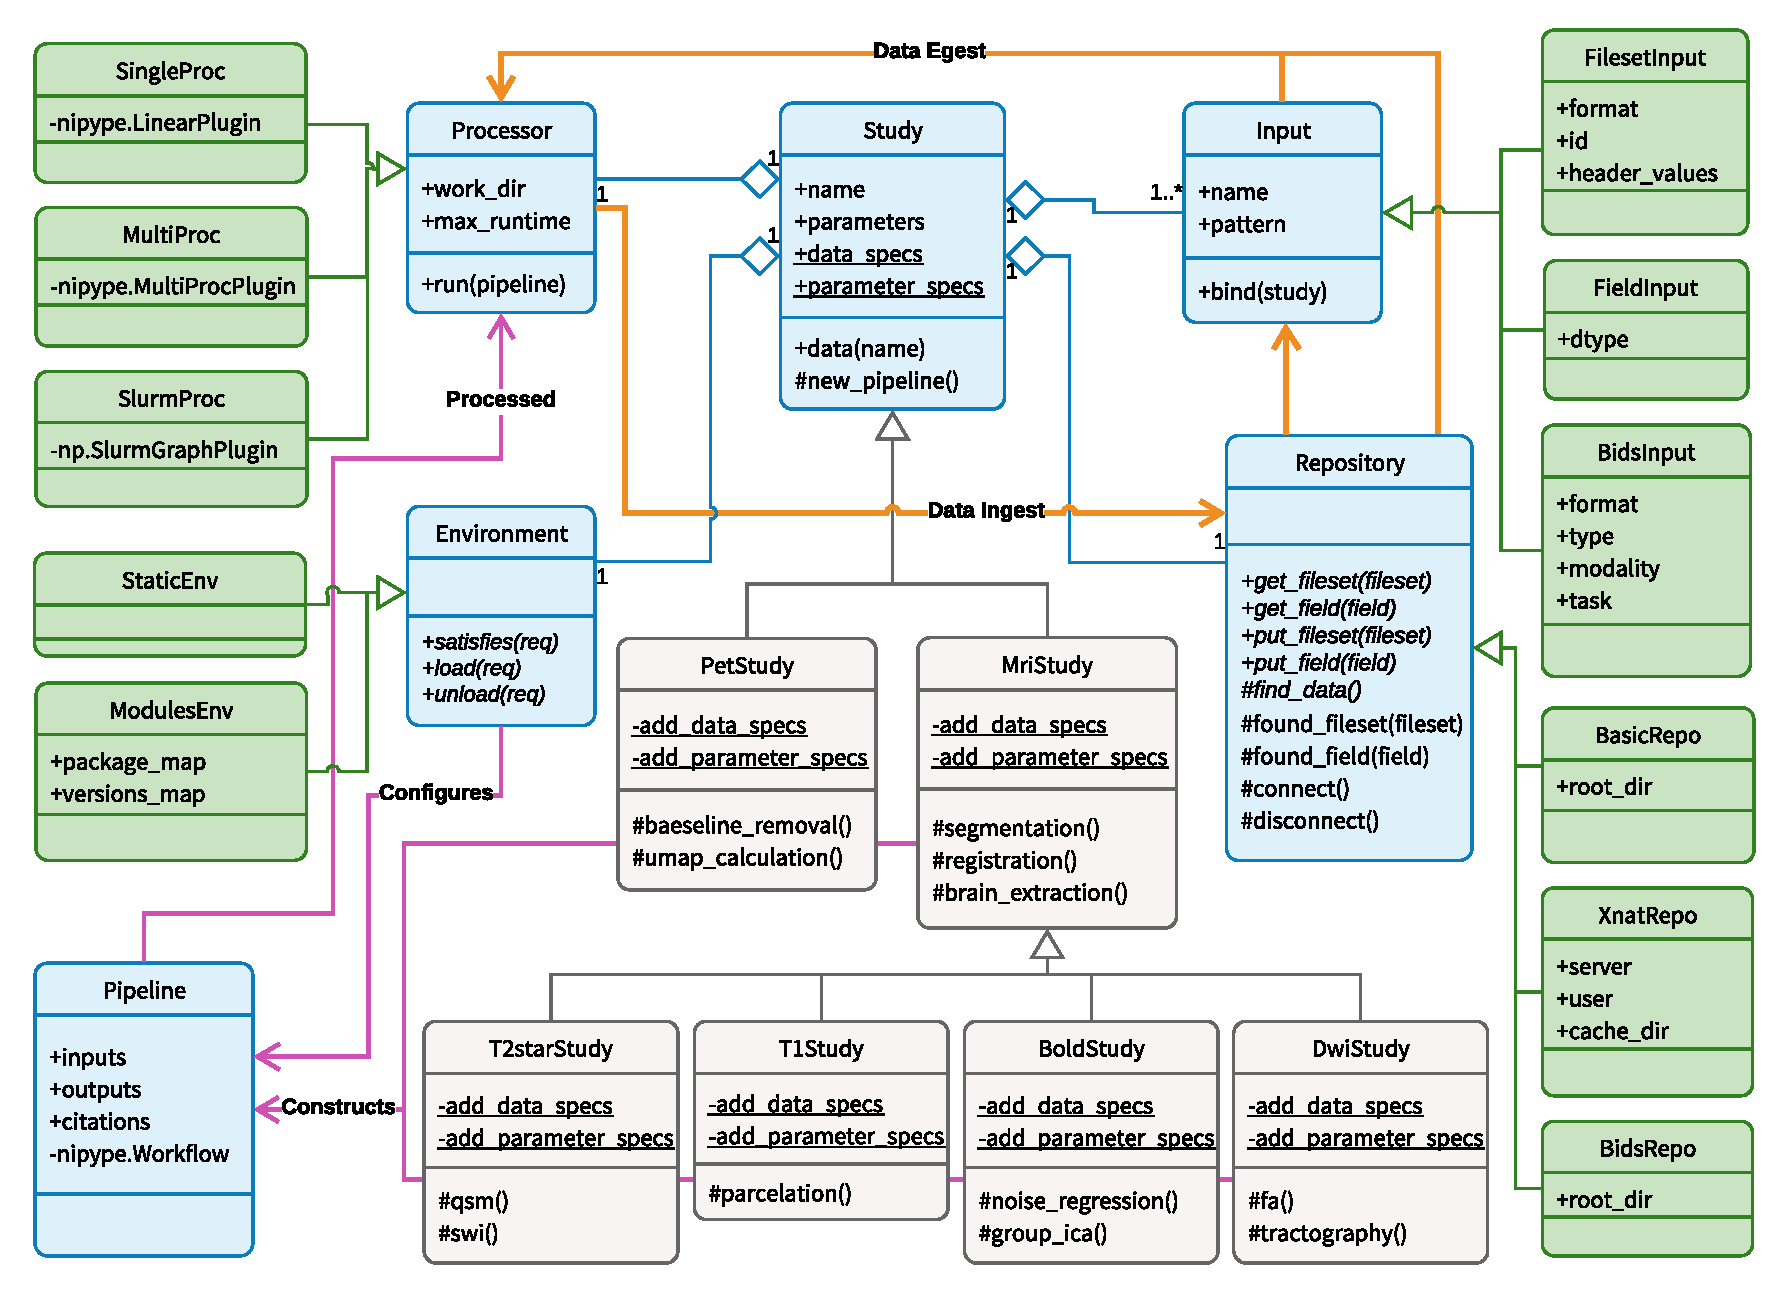
\includegraphics[width=\textwidth]{figures/full_arcana_uml}
  \caption{Detailed Unified Modelling Language (UML) diagram of
information flow in the Arcana framework. Boxes: Python classes
(blue=core, green=interchangeable modules, grey=example
specialisations). Arrows: orange=data, magenta=workflow description,
diamond=aggregated-in, triangle=subclass-of. Calling \emph{data(name)}
on a Study subclass constructs the requisite pipelines (as specified in
\emph{Study.data\_specs}) to produce the requested data, and sends them
to the \emph{Processor} to be processed. Data is selected by
\emph{Selector} objects, pulled to the compute environment to be
processed, and then the derivatives are pushed back to the repository.
Repositories can be of plain directories, or BIDS or XNAT repositories}
\label{fig:full_uml}
\end{center}
\end{figure*}

Each Study object is assigned a name, which is used to differentiate its
results from alternative analyses on the same dataset (e.g. by different
members of a lab). Parameters are set on initialisation of the Study
object along with the range of subject and visit IDs to be included in
the analysis (if they are not provided then all IDs are included). The
remaining arguments passed to the Study object initialisation are the
Repository and Processor modules and a list of \emph{Selector} objects
to select input datasets from the repository (Figure 8).

\begin{figure}
\lstinputlisting[language=Python]{listings/example_application.py}
\caption{Example application of Study class to a dataset stored in an XNAT
repository. Once the Study object has been initialised potential
derivatives of the Study can be requested, and will be generated and
stored in the repository if already present.}
\label{list:study_application}
\end{figure}

\hypertarget{repository-modules}{%
\subsubsection{Repository modules}\label{repository-modules}}

In Arcana, repository access is encapsulated within modular
\emph{Repository} objects to enable switching between different
repositories and repository types at analysis ``application time''
(Figure 2). There are currently three supported repository types, XNAT
\cite{marcus_extensible_2007}, BIDS \cite{gorgolewski_brain_2016} and a simple
``directory'' format, which are encapsulated by \emph{XnatRepository},
\emph{BidsRepository}, and \emph{DirectoryRepository} classes
respectively.

In its most basic form, a directory repository is just a file system
directory with separate subdirectories for each subject in the study,
with subject IDs taken from the subdirectory names. If the study has
more than one visit then nested subdirectories for each visit are
required in the subject subdirectories. Note that the directory
repository is similar to the BIDS format, however, there are no naming
conventions in the directory repository, which enables prototyping and
testing of analyses on loosely structured data.

Derivatives are stored by their specification name in a study-specific
namespaces to avoid clashes with separate analyses. In directory
repositories this namespace is a subdirectory named after the study
nested within each visit subdirectory if present or subject subdirectory
otherwise. In BIDS repositories, the namespace is a subdirectory of the
\emph{derivatives} directory, again named after the study. In XNAT
repositories, derivatives for each session are stored in separate
\emph{MrSession} objects alongside the primary session underneath its
\emph{Subject}, and are named
\emph{\textless{}primary-session-name\textgreater{}\_\textless{}study-name\textgreater{}}
(Table 1).

Derived filesets are stored with the format specified in the study's
data specification. In plain-directory and BIDS repositories, fields are
stored in a single JSON file named `\_\_fields\_\_.json' in each derived
session, and on XNAT they are stored in custom fields of the derived
session. Provenance is stored in a `\_\_prov\_\_' sub-directory (dataset
on XNAT) of the derivatives directory (MrSession on XNAT) in separate
JSON files for each pipeline named after the pipeline (Table 1).

Summary data (i.e. with \emph{per\_subject}, \emph{per\_visit}, and
\emph{per\_study} frequencies\emph{)} are stored in specially named
subjects and visits (e.g. `all'), the names for which are specified when
the repository is initialised. For example, given in plain-directory
repository using all as the summary name for both subjects and visits,
per\_subject data for `subj1' would be stored at
\emph{\textless{}root\textgreater{}/subj1/}all, per\_visit data for
`visit1' in \emph{\textless{}root\textgreater{}/}all\emph{/visit1},
and per\_study data in \emph{\textless{}root\textgreater{}/}all/all
(Table \ref{tbl:repo-structure}).

\begin{table}
\caption{Storage locations of derived data for each repository
type. Derivatives are stored in separate namespaces for each Study
instance to enable multiple analyses on the same datasets with different
parameterisations. Where `...' is the location of the
directory or MrSession that holds the derivatives, \emph{subj} = subject ID, \emph{vis} = visit ID,
\emph{study} = name of the Study instance, and \emph{pl} = name
of pipeline.}
\label{tbl:repo-structure} 
\begin{tabular}{llll}
\hline\noalign{\smallskip}
\textbf{Type} & Plain-directory & BIDS & XNAT  \\
\noalign{\smallskip}\hline\noalign{\smallskip}
\textbf{Derivatives} & /\emph{subj}/\emph{vis}/\emph{study} & /derivatives/\emph{study}/\emph{subj}/\emph{vis} & /\emph{subj}/\emph{vis}\_\emph{study}\\
\textbf{Fields} & \D/\_\_fields\_\_.json & \D/\_\_fields\_\_.json & MrSession XML \\ 
\textbf{Provenance} & \D/\_\_prov\_\_/\emph{pl}.json & \D/\_\_prov\_\_/\emph{pl}.json & \D/\_\_prov\_\_/\emph{pl}.json \\
\noalign{\smallskip}\hline
\end{tabular}
\end{table}

Each study can only have one repository in which derivatives are stored.
However, a study can draw data from multiple auxiliary repositories,
which are specified in the inputs passed to the study. When using
multiple input repositories, subject and visit IDs will often need to be
mapped from their values in the auxiliary repositories to the ``ID
space'' of the study. This mapping is specified using \emph{IdMapper}
objects passed to \emph{subject\_id\_map} and \emph{visit\_id\_map}
keyword arguments during initialisation of a repository.

New repository modules for additional repository types can be
implemented by extending the Repository abstract base class and
implementing a small set of methods (Table 2).

\begin{table}
\caption{Abstract methods in the base Repository class that
need to be implemented by platform-specific sub-classes.}
\label{tbl:abstract-repo-methods} 
\begin{tabular}{ll}
\hline\noalign{\smallskip}
\textbf{Method name} & Function \\
\noalign{\smallskip}\hline\noalign{\smallskip}
find\_data() & Queries repository to find all existing filesets and
fields \\
get\_fileset(Fileset) & Caches file-set (if necessary) and returns the file path. \\
get\_field(Field) & Retrieves and returns the value of the field from
the repository \\
put\_fileset(Fileset) & Inserts file-set into the repository and updates cache. \\
put\_field(Field) & Inserts the value of the Field into the repository \\
connect() & Opens a connection to the repository (optional). \\
disconnect() & Closes connection to repository (optional)\\
\noalign{\smallskip}\hline
\end{tabular}
\end{table}

\subsubsection{Study inputs}
\label{study-inputs}

While derivatives generated by a Study object are named in accordance
with the data specification of the Study class, arbitrary naming
conventions can be used for input datasets and fields to allow for
heterogeneity in acquisition procedures. A selection stage is therefore
necessary to match input data to appropriate entries in the data
specification table of the Study class. The criteria for this selection
is passed to the Study object at instantiation and is required to match
exactly one fileset or field in every session included in the study.

Selection criteria are specified by list of \emph{FilesetSelector} and
\emph{FieldSelector} objects provided to the \emph{inputs} argument of
the Study initialisation method. Matching is typically performed on file
names (dataset labels for XNAT repositories), and field names. If the
names are inconsistent across the study then regular expressions can be
used instead of exact matches by passing \emph{is\_regex=True} when
initialising the Selector. Additional criteria can be used to
distinguish cases where multiple filesets in the session match the
pattern provided, such as DICOM header values, or when using an XNAT
repository, the order and ID of the dataset.

Inputs can be drawn from auxiliary repositories by providing alternative
Repository instances to the \emph{repository} keyword of the Selector.
Care should be taken to ensure that the subject and visit ID schemes
will map correctly to that of the primary repository (see
\emph{Repository modules}). If the primary repository is empty (i.e. all
inputs come from auxiliary repositories) then explicit
\emph{subject\_ids}, \emph{visit\_ids} need to be provided and the
\emph{fill\_tree} flag set when initialising the Study.

If the data to select has been derived from an alternative study, then
the name of the alternative study can be passed to the
\emph{from\_study} keyword argument provided to the selector. There are
no restrictions on selecting any data, derived or otherwise, to match
acquired or derived specifications. For example, it is possible to
deliberately skip analysis steps by selecting an output of an early step
in a previous run as a match for a later derived spec although this is
not recommended as standard practice.

Specific files and fields that are not stored within a repository can be
passed as inputs in \emph{FilesetCollection} and \emph{FieldCollection}
objects. Collection objects reference an entry in the data specification
table and contain a single Fileset or Field for every session (or
subject/visit/study depending on the frequency of the corresponding data
spec). Collection objects can be used to pass reference atlases and
templates as inputs to analyses. They can also be set as the ``default
input'' for a data spec using the \emph{default\_input} keyword
argument. For the sake of portability, default inputs should be
restricted to data in publically accessible repositories or included in
standard software packages (e.g. FSL).

When using BIDS repositories, the selection stage is typically already
included in the data specification (see \emph{Data and parameter
specifications)} so inputs do not need to be provided to the
initialisation of the Study. However, BidsSelector and
BidsAssociatedSelector objects can be provided to override the default
selections is required.

\subsubsection{Processor modules}
\label{processor-modules}

Processor modules control how and where pipelines generated by a Study
are executed. There currently four Processor modules implemented in
Arcana: \emph{LinearProcessor}, \emph{MultiProcProcessor},
\emph{SlurmProcessor} and \emph{SgeProcessor}, which wrap the
correspondingly named Nipype execution plugins. The main task performed
by the processor, as separate from the Nipype execution plugin it wraps,
is to determine which pipelines need to be run and link them into a
single workflow. Since this logic is implemented in the Processor
abstract base class, wrapping additional Nipype plugins as required is
trivial.

A processor is used internally by a Study instance to execute pipelines
to derive derivatives requested from the data specification by the
\emph{Study.data(name{[}, name,...{]})} method (Figure 2). The first
step in this procedure is to query the repository tree for all data and
provenance associated with the study. Sessions for which the requested
outputs of the pipeline are already present in the repository are
excluded from the list to process. For the remaining sessions to
process, inputs of the pipeline that are derivatives themselves are
added to the stack of requested derivatives. This procedure is repeated
recursively until there are no sessions to process or all inputs to the
pipeline are study inputs at a given depth.

When a pipeline is processed it is connected to \emph{Source} and
\emph{Sink} nodes, which get and put the pipeline inputs and outputs
from and to a repository, respectively. Separate source and sink nodes
are used for each data frequency (i.e. per-session, per-subject,
per-visit, per-study). If implicit file format conversion is required
(i.e. the input or output format differs from the data specification)
then additional format converter nodes are inserted after the source
nodes or before the sink nodes. Iterator nodes that iterate over the
required subjects and visits are connected to the sources, and report
nodes that join over subjects and visits are connected to the sink
nodes. Report nodes of upstream pipelines are connected to downstream
iterator nodes to create a single workflow, which is then executed using
the Nipype execution plugin.

Software versions are managed by the processor if environment modules
\cite{furlani_modules:_1991} are installed on the system. These are loaded and
unloaded before the interface of a workflow node is run based on the
requirements specified for the node during construction of the pipeline
(see \emph{Pipeline constructors}. Maps from requirement names to
module names in the processing environment can be passed to the
Processor at initialisation. For plugins that submit jobs to HPC
schedulers (e.g. SLURM, SGE), node memory and wall-time requirements are
inserted into jobscripts where required.

Provenance is stored for each pipeline run alongside the generated
derivatives and consists of: parameter values used by the pipeline,
software versions used by the pipeline, a graph representation of the
underlying Nipype workflow, checksums of inputs, version of Arcana used,
version of Nipype used, subject and visit IDs used by study.

For subsequent analyses, changes w.r.t. Any of the stored values, with
the exception of subject and visit IDs, will be flagged as a mismatch.
Subject or visit IDs only flag a mismatch if any of the inputs, or
inputs of upstream pipelines, are per-visit or per-subject,
respectively, or per-study. How provenance mismatches are handled by the
study is determined by the \emph{reprocess} flag, which is passed to the
Study on initialisation (Table 3).


\begin{table}
\caption{Effect of the \emph{reprocess} flag value on the
behaviour of the study when existing derivatives are found that were
derived with mismatching inputs and parameters.}
\label{tbl:reprocess-flag} 
\begin{tabular}{ll}
\hline\noalign{\smallskip}
\textbf{Reprocess value} & \textbf{Behaviour on provenance mismatch} \\
\noalign{\smallskip}\hline\noalign{\smallskip}
False (default) & Raises an exception \\
True & Mismatching derivatives will be reprocessed \\
`ignore' & Mismatches are ignored \\
`ignore\_versions' & Ignore versions, otherwise raise exception \\
`ignore\_versions\_true' & Ignore versions, otherwise the derivative will be reprocessed \\
\noalign{\smallskip}\hline
\end{tabular}
\end{table}

Additionally, a time limit can be passed to the
\emph{reprocess\_time\_limit}, and if the estimated time to reprocess
all the required sessions is less than the time limit they will be
reprocessed and otherwise an exception will be raised.

\section{Results}
\label{results}

The Arcana framework is distributed as a publicly available software
package via GitHub
(\href{http://github.com/MonashBI/arcana}{{http://github.com/MonashBI/arcana}})
and the Python Package Index (PyPI)
(\href{https://pypi.org/project/arcana/}{{http://pypi.org/project/arcana/}}).
Study classes for T1, T2* and diffusion weighted MRI data have been
implemented as part of the \emph{Biomedical imAgiNg ANAlysis (Banana)}
package
(\href{https://github.com/MonashBI/banana}{{http://github.com/MonashBI/banana}};
\href{http://pypi.org./project/banana}{{http://pypi.org./project/banana}}).
All three classes, \emph{T1wStudy}, \emph{T2starwStudy} and
\emph{DmriStudy}, inherit generic image analysis methods, such as
registration and brain extraction, from the base class \emph{MRIStudy}.
The T1Study and T2starStudy classes are aggregated into the
\emph{T2starwT1wStudy} MultiStudy class to combine analysis of T2* and
T1-weighted contrasts.

The DmriStudy class implements diffusion tensor metrics, FA and ADC, as
well as global tractography using streamlines tracking from the MRtrix
toolbox \cite{tournier_improved_2010,tournier_mrtrix:_2012} (Figure 9).

\begin{figure*}
  \begin{center}
    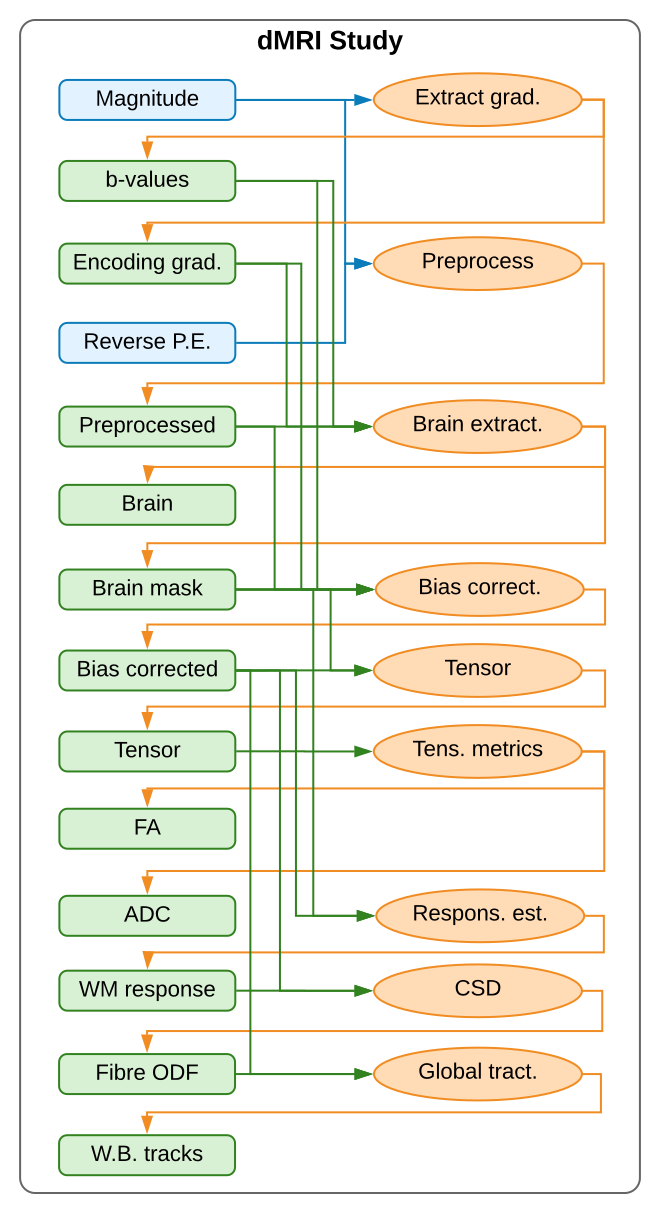
\includegraphics[width=0.55\textwidth]{figures/dmri_study}
  \caption{Example diffusion MRI (dMRI) study, which can derive
tensor metrics, fractional anisotropy (FA) and apparent diffusion
coefficient (ADC) as well as streamlines fibre tracking. Blue boxes:
acquired (input) data (filesets or fields). Green boxes: derivatives.
Orange ovals: pipelines. Blue and green arrows: acquired and derived
inputs to pipelines, respectively. Orange arrows: outputs of pipelines.
The dMRI magnitude image is preprocessed for motion correction and EPI
distortions masked and bias corrected. From the bias corrected image two
branches of analysis can be performed using the same intermediate
derivatives: FA and ADC and/or streamlines fibre tracking.}
\end{center}
\label{fig:dmri_study}
\end{figure*}

The \emph{T2starwT1wStudy} class implements an algorithm to generate
\emph{composite vein images} from the combination of QSM and SWI
contrasts derived from the T2*-weighted acquisition with an vein atlas
registered to the T1-weighted acquisition \cite{ward_combining_2018} (Figure 10).

\begin{figure*}
  \begin{center}
    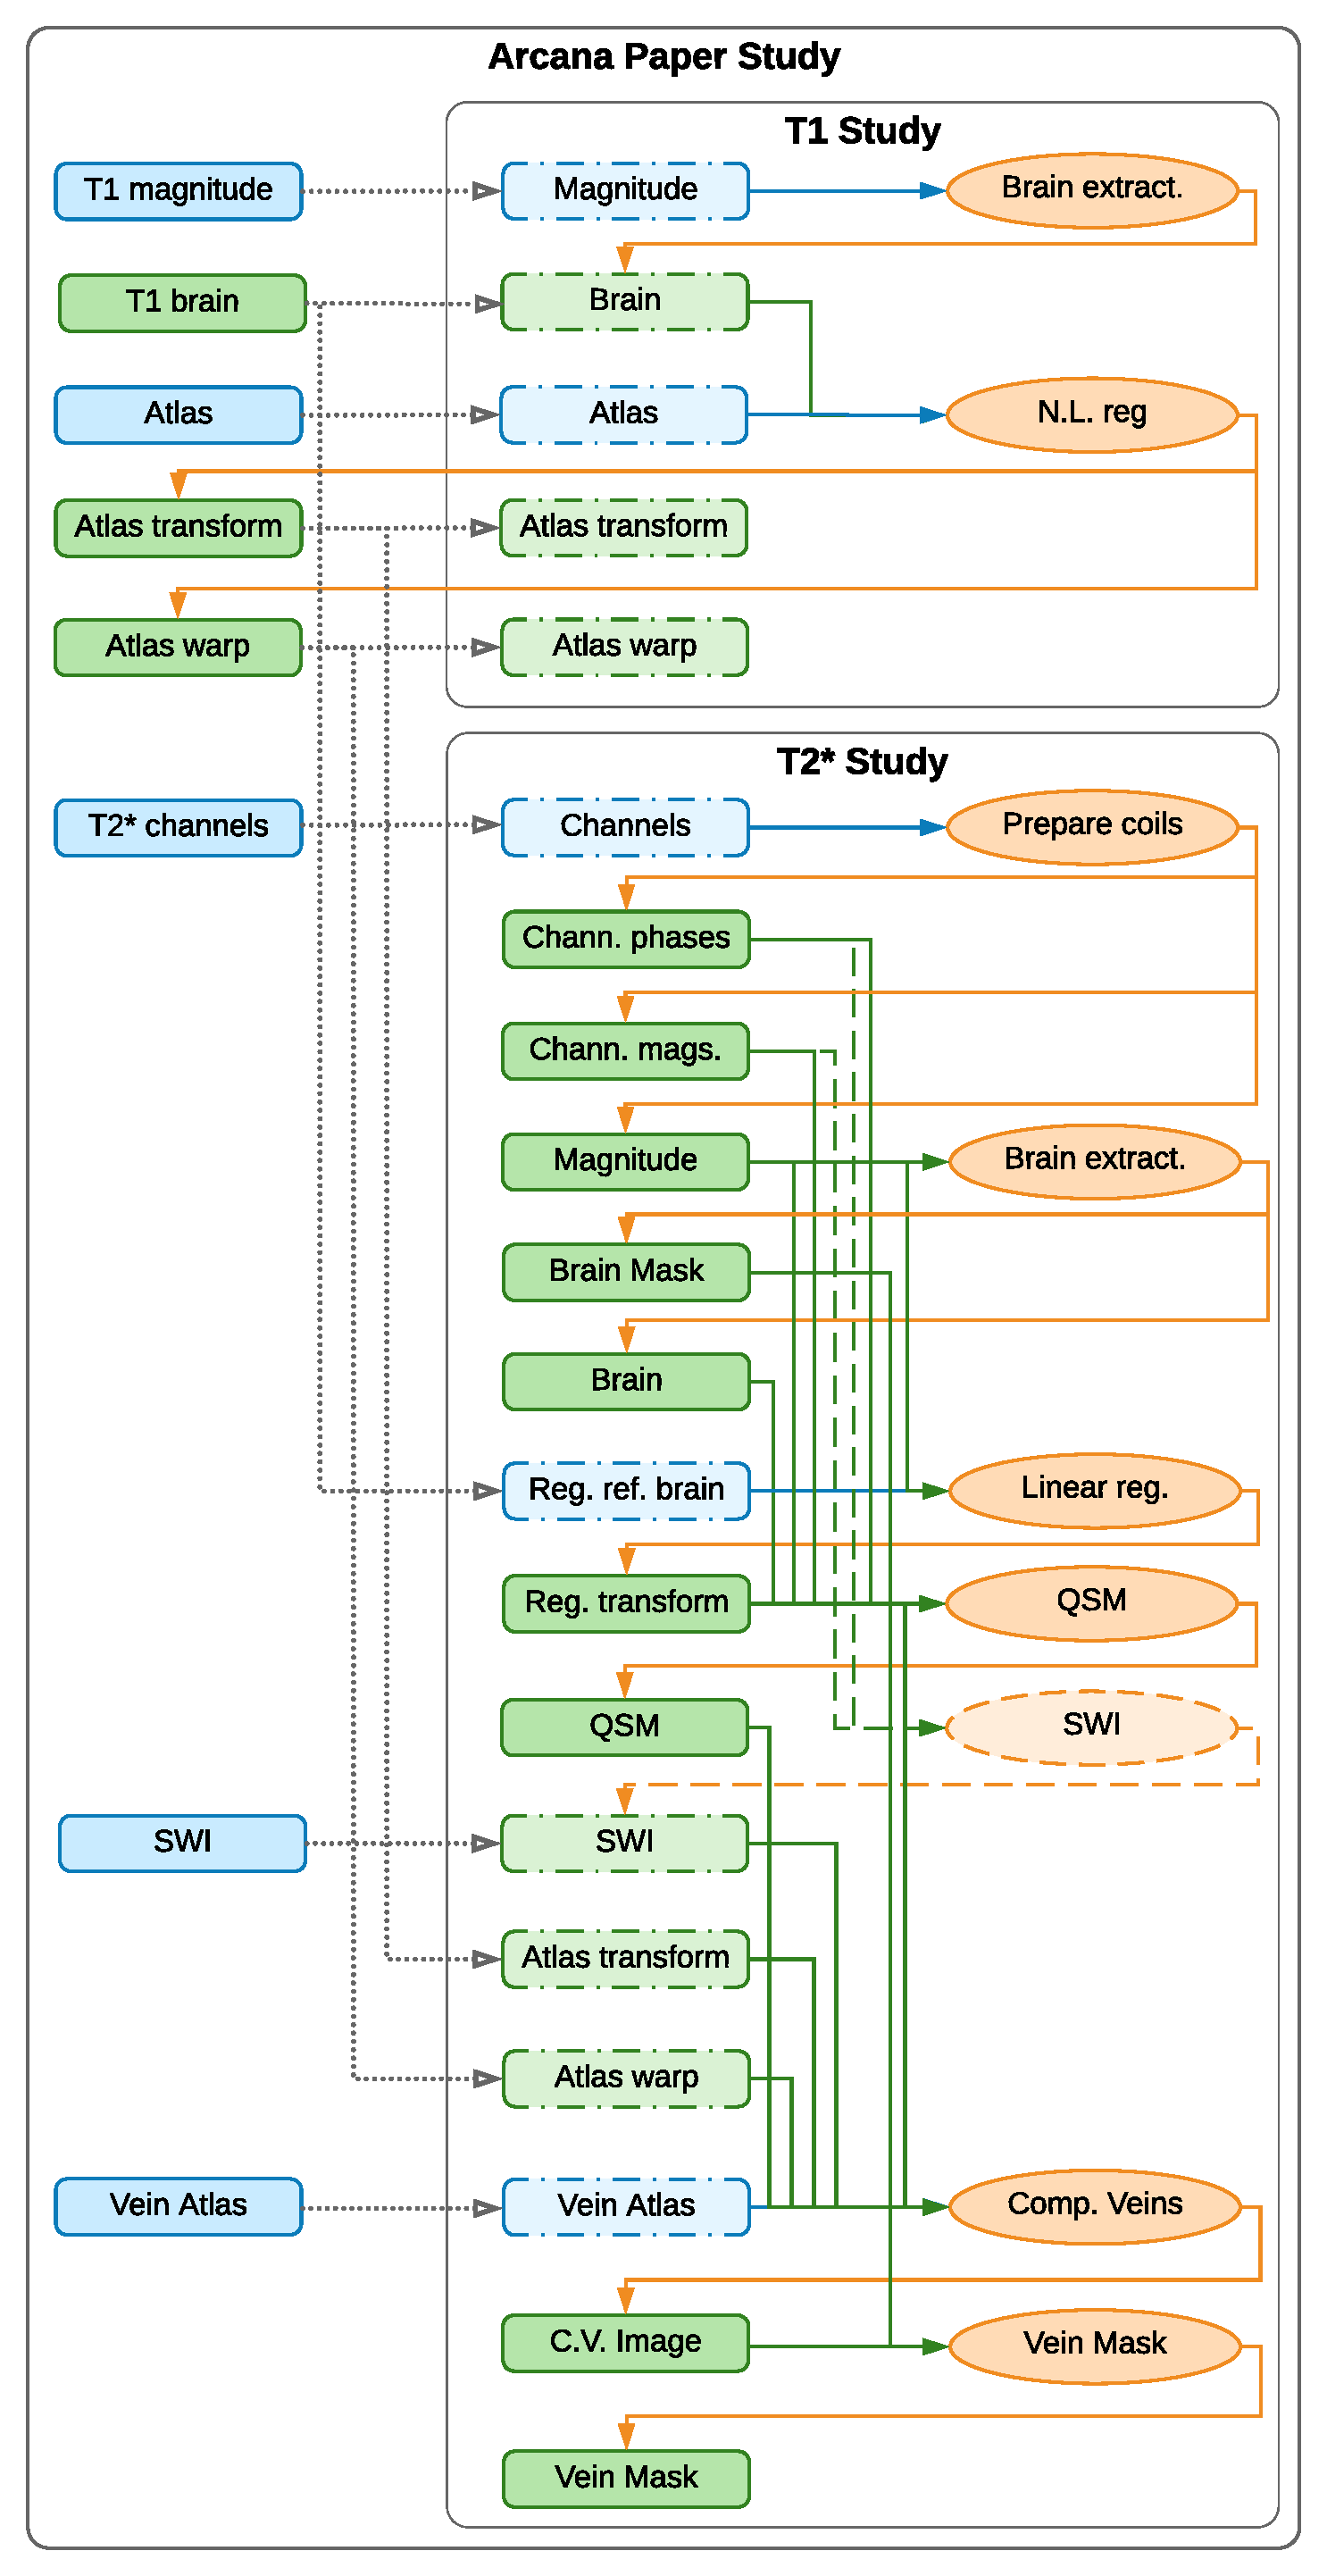
\includegraphics[width=0.775\textwidth]{figures/t2star_t1_study}
  \caption{Combined T2*-weighted/T1-weighted multi-study,
which can derive vein masks by combining Quantitative Susceptibility
Mapping (QSM) and Susceptible Weighted Imaging (SWI) contrasts with a
manual atlas. Blue boxes: acquired (input) data (filesets or fields).
Green boxes: derivatives. Orange ovals: pipelines. Blue and green
arrows: acquired and derived inputs to pipelines, respectively. Orange
arrows: outputs of pipelines. Dashed boxes represent data specifications
in a sub-study that are present in the global namespace and mapped into
the sub-study space, and dotted arrows the mappings. The acquired
T1-weighted image is mapped to both the \emph{magnitude} spec of the
T1-weighted sub-study and the \emph{registration reference} spec of the
T2*-weighted sub-study. The nonlinear transformation from subject to
atlas space are mapped from the T1-weighted sub-study and combined with
the linear registration between T1-weighted and T2*-weighted images, QSM
and SWI images mapped from the T2*-weighted sub-study to produce the
composite-vein image. The brain mask from the T1-weighted sub-study is
combined with the composite vein image to produce the vein mask.}
  \end{center}
\label{fig:t2star_t1_study}
\end{figure*} 

The DiffusionStudy and T2starT1Study classes are further aggregated in
turn into a single MultiStudy class for the results section of this
manuscript\emph{, ArcanaPaper}, (Figure S.1-5). Methods are implemented
in ArcanaPaper to generate and display the derivative images in Figures
11, 12, and 13.

To test the analysis workflows implemented in ArcanaPaper, a healthy
volunteer was scanned using a 3T Siemens Skyra with a 32-channel head
and neck coil. The protocol was a T1-weighted MPRAGE (1mm contiguous,
matrix size 256x240x192, FOV 256x240x192, TE = 2.13ms, TR, = 2300ms, TI
= 900ms, bandwidth=230Hz/pixel), GRE (1.8 mm contiguous, matrix size
256x232x72, FOV 230x208x130, TE = 20ms, TR, = 30ms,
bandwidth=120Hz/pixel), diffusion MRI (1.2 mm contiguous, matrix size
110x100x60, FOV 256x240x192, TE = 95ms, TR, = 8200ms, 33 diffusion
directions with b=1500 mm2/s and 3 b=0, bandwidth=781Hz/pixel)
(\textbf{cite Lifespan paper ??}). Methods for Figure 11, 12, and 13 in
the ArcanaPaper class were applied to the acquired dataset to using the
\emph{SlurmProcessor} to submit jobs to the the MASSIVE HPC cluster
\cite{goscinski_multi-modal_2014} in order to generate the figures.

Figure \ref{fig:veins} displays composite vein images and vein masks for the healthy
volunteer along with the SWI and QSM intermediate derivatives and the
input vein atlas. The derived vein images are comparable to those
generated by the original implementation \cite{ward_combining_2018}. The complete
workflow took ?? min to complete over ?? compute cores.

\begin{figure*}
  \begin{center}
    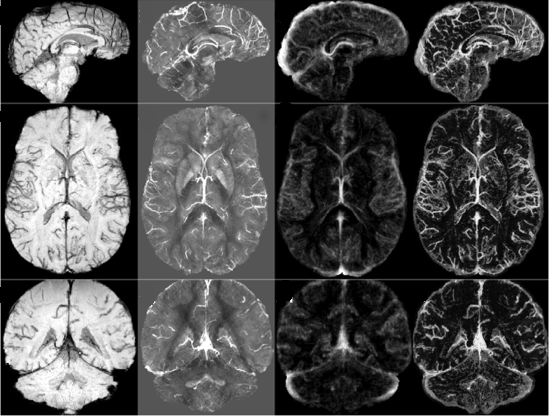
\includegraphics[width=\textwidth]{figures/veins}
  \caption{Vein image (\emph{right column}) constructed by
combining susceptibility weighted imaging (SWI) (\emph{left column}),
quantitative susceptibility mapping (QSM) (\emph{left-middle column})
and a vein atlas from manual tracings (\emph{right-middle column}).
\emph{Top row}: sagittal slices. \emph{Middle row}: axial slices.
\emph{Bottom row}: coronal slices.}
  \end{center}
\label{fig:veins}
\end{figure*}

Figure \ref{fig:fa_adc}  displays the FA and ADC maps derived from the diffusion MRI
acquisition. The FA map shows high intensity in known white matter
tracts and low intensities in known grey matter regions. The ADC map
shows high intensity in cortical spinal fluid and low intensity through
the rest of the brain.

\begin{figure*}
  \begin{center}
    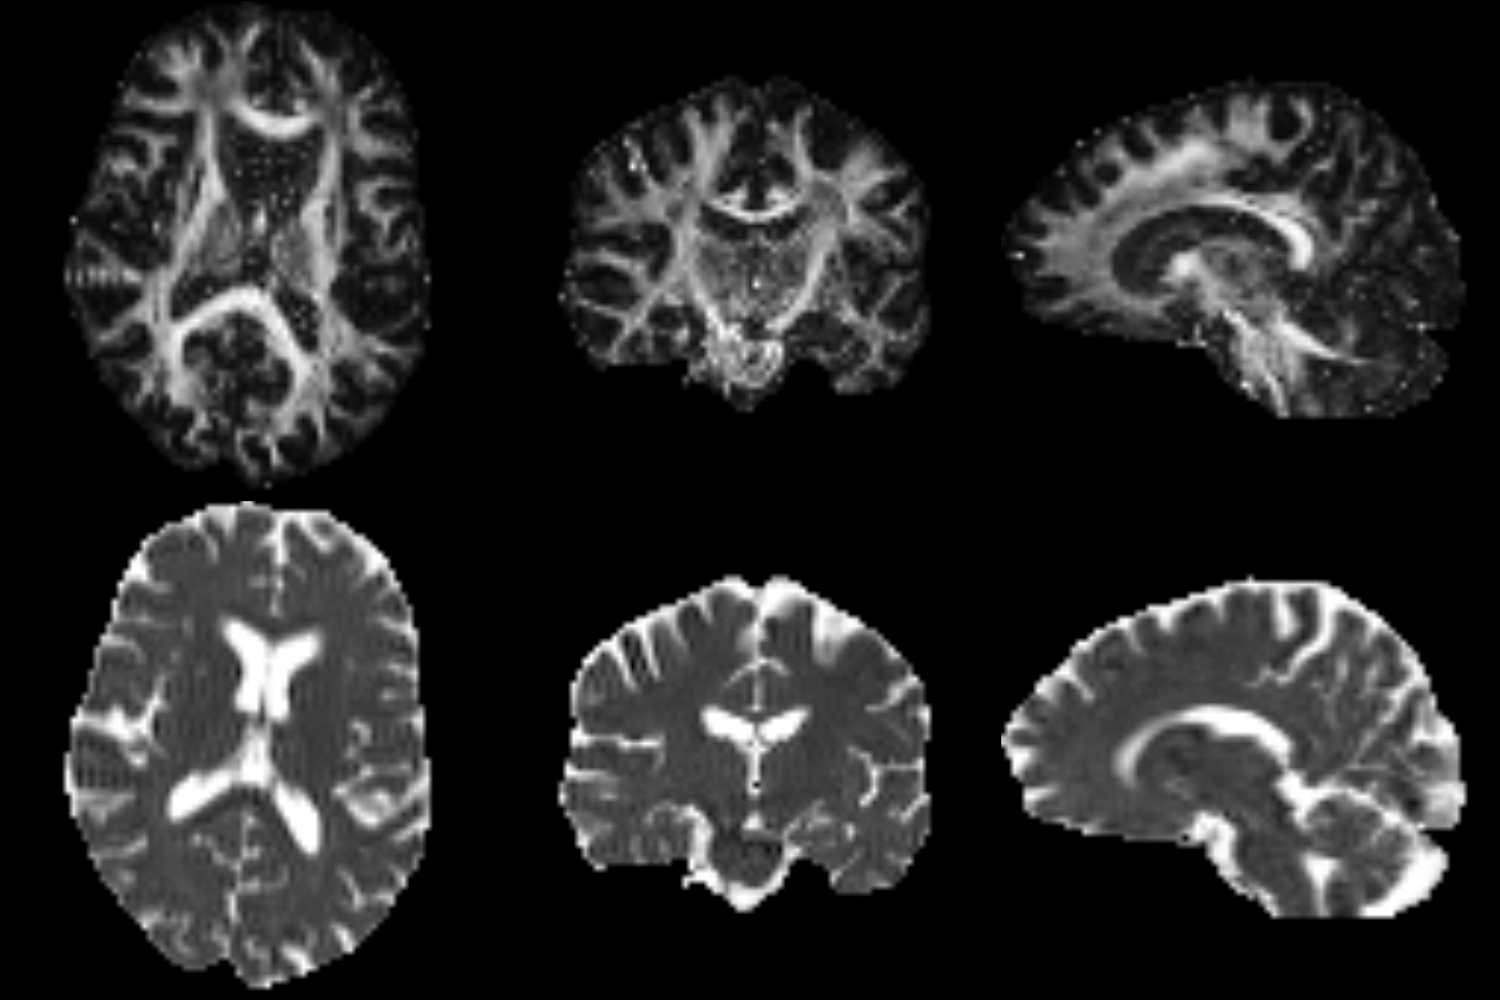
\includegraphics[width=\textwidth]{figures/fa_adc}
  \caption{Fractional Anisotropy (FA) \emph{(top row)} and
Apparent Diffusion Coefficient (ADC) (\emph{bottom rowI)} derived from
diffusion MRI data. \emph{Left column:} axial midline slices.
\emph{Middle column:} coronal midline slices. \emph{Left column}:
sagittal midline slices.}
  \end{center}
\label{fig:fa_adc}
\end{figure*}

Figure \ref{fig:tractography} displays the global tractography derived from the dMRI
acquisition. The streamlines follow well known white matter tracts such
as the cortico-spinal, fasciculus and corpus callosum. Intermediate
derivatives derived for the FA and ADC analysis, including the
preprocessed and bias-corrected dMRI image and a whole brain mask, were
reused in the generation of the streamlines reducing the time taken to
produce the tractography results from ?? to ??.

\begin{figure*}
  \begin{center}
    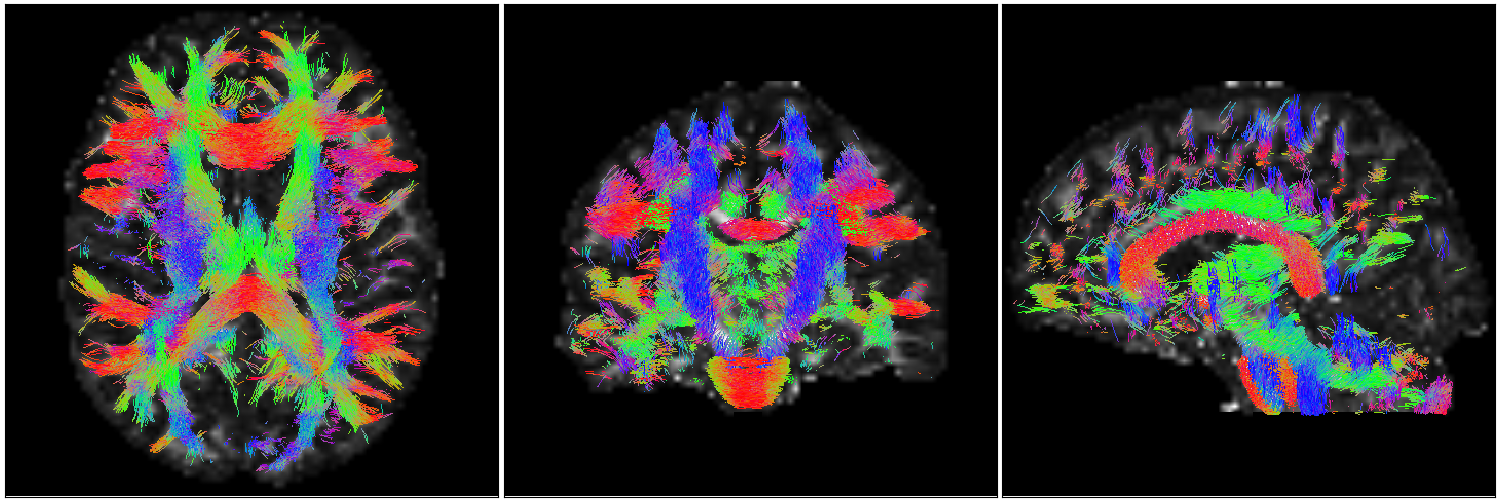
\includegraphics[width=\textwidth]{figures/tractography}
  \caption{Global tractography performed using the MRtrix
toolbox. Probabilistic streamlines generated with the iFOD2 algorithm
from fibre Orientation Distribution Function (fODF) estimated from
diffusion MRI datasets using Constrained Spherical Deconvolution (CSD).
Streamlines are colour-encoded by orientation: green=anterior-posterior,
blue=inferior-superior, red=left-right. \emph{Left panel:} axial midline
slice. \emph{Middle panel:} coronal midline slice. \emph{Left panel}:
sagittal midline slice.}
  \end{center}
\label{fig:tractography}
\end{figure*}

\section{Discussion}
\label{discussion}

We present Arcana, a software framework to facilitate the development of
comprehensive analysis suites for neuroimaging data that implement
complete workflows from repository data to publication results. The
encapsulation of repository data and workflow generation in Arcana
enables researchers to create robust workflows while focussing on the
core logic of their analysis. Arcana's modular pipeline and OO
architecture promotes code reuse between different workflows by
facilitating the sharing of common segments (e.g. registration,
segmentation). The clear separation of analysis design from its
application leads to portable workflows, which can be applied to
datasets stored in a number of storage systems. In addition, the
management of intermediate derivatives, provenance and software
versioning, coupled with ability to submit jobs to HPC clusters, enables
workflows implemented in Arcana to scale to large datasets. Arcana
thereby enables researchers to quickly prototype analysis suites on
local workstations that can be deployed on enterprise-scale
infrastructure without modification.

Software frameworks \cite{yacoub_pattern-oriented_2004} have been successful in
improving code quality and efficiency of development in a variety of
contexts \cite{moore_professional_2008,white_hadoop:_2012,abadi_tensorflow:_2016}. By
factoring out common elements, only features that are specific to the
given application need to be implemented by the analysis designer, and
the common elements become battle hardened through repeated use. Arcana
handles many of the menial tasks involved with workflow implementation,
such as data retrieval and storage, format conversions, and provenance,
reducing the time and effort required to implement robust workflows from
acquired data to publication results.

An oft-repeated mantra in the open-source software movement dubbed
Linus' Law is that "given a large enough beta-tester and co-developer
base, almost every problem will be characterized quickly and the fix
obvious to someone" or more compactly, "given enough eyeballs, all
\href{https://en.wikipedia.org/wiki/Software_bug}{bugs} are shallow"
\cite{raymond_cathedral_1999}. Given the size of the neuroimaging research community,
there are a large number of potential beta-testers and co-developers.
However, it has been difficult for researchers to collaborate on the
same code base due to slight differences in acquisition protocols,
storage conventions, researcher preferences, and study requirements.

The flexibility and portability of the Arcana framework increases the
feasibility of community collaborations on workflow implementations. The
improvement of code quality in larger community efforts, due to more
eyeballs to detect and fix errors, has the potential to form a
reinforcing cycle where in more developers are attracted to the project.
To these ends, the Banana code repository on GitHub
(\url{http://github.com/MonashBI/banana.git}) is proposed as a code base
for communal development of neuroimaging workflows in Arcana.

A level of proficiency in Python OO design is required to design new
analyses in Arcana, which may preclude inexperienced programmers.
However, only a basic knowledge of Python is required to apply existing
analyses to new datasets. Furthermore, a number of example Study classes
have been implemented, which can guide the hand of analysis designers.
Arcana imposes a consistent structure on workflows implemented within
it, making the code easier to understand for developers who are familiar
with the framework. In addition, class inheritance provides a manageable
way to adapt and extend to existing analyses and highlights where
modified analyses differ from standard procedures.

MR contrast-specific analyses are implemented in NiAnalysis via a chain
of successively specialised Study sub-classes (e.g.
MRI\textgreater{}EPI\textgreater{}dMRI) to enable generic processing
steps (e.g. registration) to be shared between classes. While not
necessary, it is recommended to create a subclass specific to the
research study in question and aggregate all related analysis within it,
since such classes can be applied to alternate datasets in order to
reproduce the exact analysis. The \emph{ArcanaPaper} class (Figure
S.1-5), which contains methods to generate all figures in the Results
section of this manuscript, is an example of this approach.

The abstraction of data and repositories in Arcana enables the same
workflow implementation to be applied to datasets stored in BIDS format
or XNAT repositories. A single code-base can therefore be containerized
into BIDS apps or XNAT pipelines without adaptation, helping to form a
bridge between the two communities of users and developers. Alternative
data storage systems \cite{,scott_coins:_2011,das_loris:_2012,book_neuroinformatics_2013}, can be integrated into Arcana by overriding a small number of
methods from the Repository abstract base class. Repository modules
could also be created for data portals such as \emph{DataLad} \cite{yaroslav_halchenko_datalad/datalad_2018} in order to take advantage of the range of platforms they support.
Implementing analyses in Arcana therefore enables researchers and
research groups to easily migrate their workflows between storage
platforms, and not risk being locked in to a particular technology.

While Arcana was primarily developed for neuroimaging datasets, it is a
general framework that could be applied to data from other fields.
However, in other contexts, the subject and visit hierarchy may no
longer make sense. In many cases it may be sufficient to map subjects
and/or visits onto alternative concepts (e.g. for meteorological data
\emph{subjects} = \emph{weather stations}, \emph{visits = observation
times}). But some cases may require a deeper data hierarchy (i.e.
greater than two), which is not currently possible in Arcana.

Ensuring that the consistent versions of external tools are used
throughout the analysis is important to avoid introducing biases due to
algorithm updates. In systems with environment modules \cite{furlani_modules:_1991}
installed, Arcana loads and unloads the required modules before and
after each node is executed. When running Arcana within a container,
environment modules and software versions can be installed inside the
container giving exact control over the versions used. To these ends, a
Docker container is available on Docker Hub,
(\href{http://hub.docker.com/r/monashbi/banana}{{http://hub.docker.com/r/monashbi/banana}}),
which can be used as a base for neuroimaging analysis containers.

While the same tools and versions should be applied across an analysis
to avoid bias, there are cases where it is desirable to rerun the same
analysis with different tools substituted at various points in the
workflow. In particular, when introducing new tools or upgrades to
existing tools, it is important to show the effect on the final results
in comparison with existing methods. Furthermore, it is typically not
clear what variability between results produced by comparable tools is
due to. Therefore, in the absence of \emph{a priori} reason to favour a
particular tool, perhaps the most rigorous approach is to rerun analyses
with different combinations of available tools and only present results
that are robust to the ``analytic noise'' (cite here?) they introduce.
Switch parameters make it straightforward to rerun analyses in Arcana
with substituted tools while controlling all other aspects of the
workflow.

Arcana's management of intermediate derivatives and provenance
guarantees that the same analysis is applied across the dataset without
necessarily requiring a complete rerun of the analysis. This guarantee
makes it feasible to process data as it is acquired over the course of
long studies, and therefore help detect any problems that might arise
with the acquisition protocol when they occur. In addition, by reusing
shared intermediate derivatives between analyses, such as the
preprocessed dMRI shared between tensor and fibre tracking workflows
(Figures 12 and 13), processing time as well as time required for manual
QC is minimised. Given analyses implemented in Arcana are also able to
be processed on HPC clusters, they scale well to large studies.

\section{Conclusion}
\label{conclusion}

By managing the complete flow of data from/to a repository with modular
components, Arcana enables complex analyses of large-scale neuroimaging
studies that are portable across a wide range of research sites. The
extensibility of analyses implemented in Arcana, coupled with the
flexibility afforded by programmatic constructuction of pipelines,
facilitates the design of comprehensive analyses by larger communities.
Larger communities of developers working on the same code-base should
make it feasible to capture the arcana of neuroimaging analysis in
templates that can be applied to a wide range of relevant datasets.

\begin{acknowledgements}
The authors acknowledge the facilities and scientific and technical assistance
of the National Imaging Facility, a National Collaborative Research
Infrastructure Strategy (NCRIS) capability, at Monash Biomedical Imaging,
Monash University. \textbf{Salary support for me ??} Early versions of the software described in the manuscript
were informed by existing software written Parnesh Raniga while
employed at Monash Biomedical Imaging.
\end{acknowledgements}

% BibTeX users please use one of
\bibliographystyle{spbasic}      % basic style, author-year citations
%\bibliographystyle{spmpsci}      % mathematics and physical sciences
%\bibliographystyle{spphys}       % APS-like style for physics
\bibliography{arcana}   % name your BibTeX data base

\end{document}
% end of file template.tex

